Track fitting and alignment makes use of many different pieces of software from conversion of data to the final NTuples for analysis. All this is documented in the general introduction to EUTelescope:
\newline
\url{https://cds.cern.ch/record/2000969/files/AIDA-NOTE-2015-009.pdf}
\newline
This manuel requires a basic understanding from the general introduction. The GBL algorithm is documented in detail here:
\newline	
\url{https://www.wiki.terascale.de/images/6/6b/Gbl_man.pdf}
\newline
Millepede is used for alignment and is documented here:
\newline
\url{http://www.desy.de/~blobel/Mptwo.pdf}
\newline


Examples are included with all installations and a step by step guide in the form of README files is provided to take a new user through the full process. All geometry files and raw data are provided and therefore run out of the box. The correct geometry after full alignment is also included with each example to aid in debugging and learning.  The examples can be found in the trunk directory and moving to jobsub/examples/GBL .

\section{Requirements}
BOOST is needed to run the additional track analysis software. This is not a prerequisite of EUTelescope at the moment and must be installed separately. Plots which come with running the processor:

\begin{description} 
\item[P-Value distributions for all fit parameters] 
\item[2D Residuals (Plane surface)] 
\item[Incidence Angles] 
\item[2D/1D kink angles] 
\item[2D Efficiency measurements] Only for DUT without consideration of timing cuts
\item[Hit maps] 
\end{description} 

Additionally a track selection processor can be used to cut on particular track properties. This only cuts on chi2 at the moment but can be easily updated to cut on other track properties. 


The gear file format is special for use with GBL and is shown in figure \ref{fig:gear} 

\begin{figure}[H]
\centering
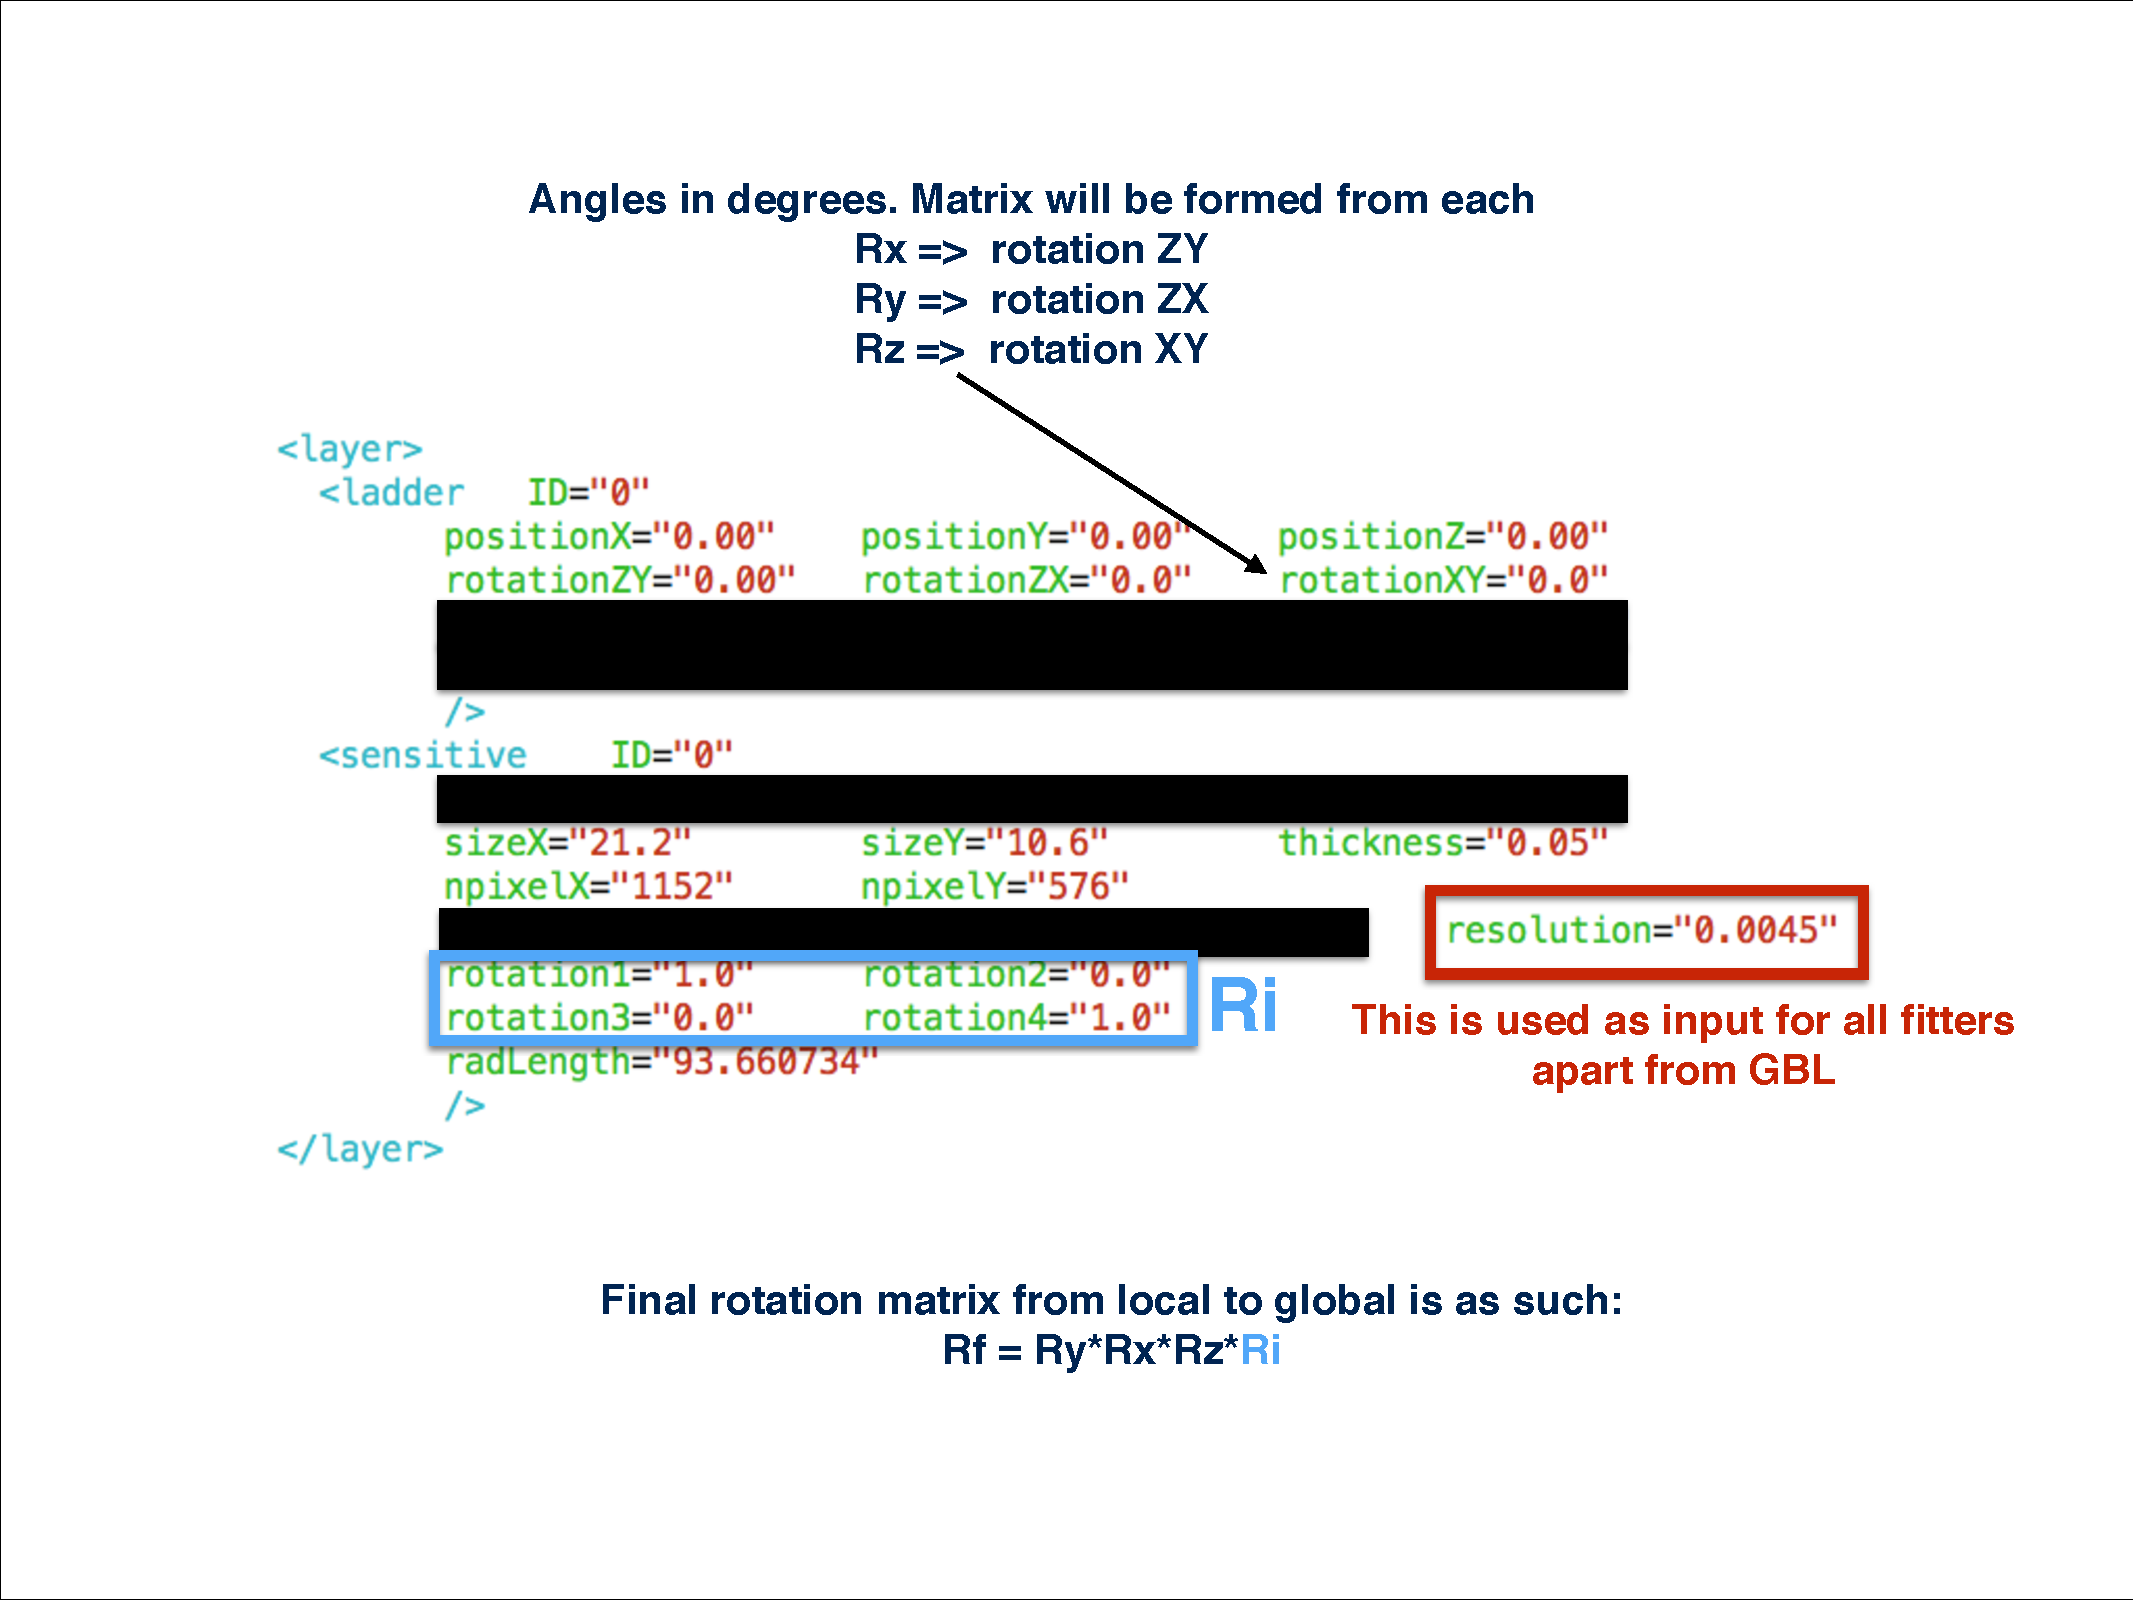
\includegraphics[width=1.0\linewidth]{figures/gear-format.pdf}
\caption{The gear format used with the GBL processor. The black lines are entries not used.}
\label{fig:gear}
\end{figure}

\section{Output format}
Many analyses require the output of the tracking data to be written in a ROOT NTuple format. Two different formats have been created which write the tracks with all clustering information to a ROOT file. Both outputs are used within the SCT example but can be used with any example with an update to the examples' steering files. 

One format was used for the analysis of ATLAS strip data for research concerning the upgrade. This has been used for detailed efficiency measurements. The other format allows the use of TBMon, a large analysis framework were additional selection and analysis can take place.



